\documentclass{article}
% \usepackage{graphicx} % Required for inserting images
\usepackage{amsmath}
\usepackage{graphicx}
\usepackage[style=ieee, url=false]{biblatex}
\usepackage{parskip} % adds a skipped paragraph
\addbibresource{jpump.bib} %Import the bibliography file

\newcommand\Mach{\mbox{\textit{Ma}}}  % Mach number
\newcommand\Tee{\mbox{\textit{TEE}}}  % Throat Entry Equation

\title{Optimizing Power Fluid in Jet Pump Oil Wells}
\author{Kaelin Ellis}
\date{September 2024}

\begin{document}

\maketitle

\section{Introduction}

Jet pumps have been installed in oils wells since the 1980's. Until recently they have been a fringe artificial lift method compared to more traditional gas lift, electric submersible pumps or plunger lift. Greater adoption of jet pumps is occurring in wells that are prone to temperature related flow assurance issues. The power fluid is heated at surface, turning the oil wells annulus and tubing into a heat ex-changer. A scaled application of multiple jet pumps oil wells will share a surface power fluid pump. The surface pump creates a finite resource of power fluid that must be distributed among all the subsurface jet pumps. The distribution creates an optimization problem, where oil rate needs to be maximized with power fluid minimization. A method is proposed in this thesis that solves the optimization problem. Should I say reservoir fluid or oil mixture? Define this term?

\section{Jet Pump Overview}

Jet pumps are very simple devices that are broken into three mechanical components and six reference locations. Figure \ref{fig:jetpump_side} provides a sketch of the geometry of a jet pump. The three components are the nozzle, throat and diffuser. The six reference locations are the suction, nozzle inlet, nozzle tip, throat entrance, throat mixture and diffuser outlet. The reservoir fluid flows to the suction, while the power fluid flows to the nozzle inlet. Both the reservoir fluid and power fluid experience an increase in velocity as they are respectively constricted through the throat entrance and nozzle tip. The increase in velocity creates a drop in pressure, allowing the two fluids to reach an equilibrium pressure. In the throat momentum is transferred from the power fluid to the reservoir and mixing occurs. The cross sectional area is increased in the diffuser, reducing the velocity and increasing the pressure. With the pressure increase the fluid can flow to surface. 

\begin{figure}
    \centering
    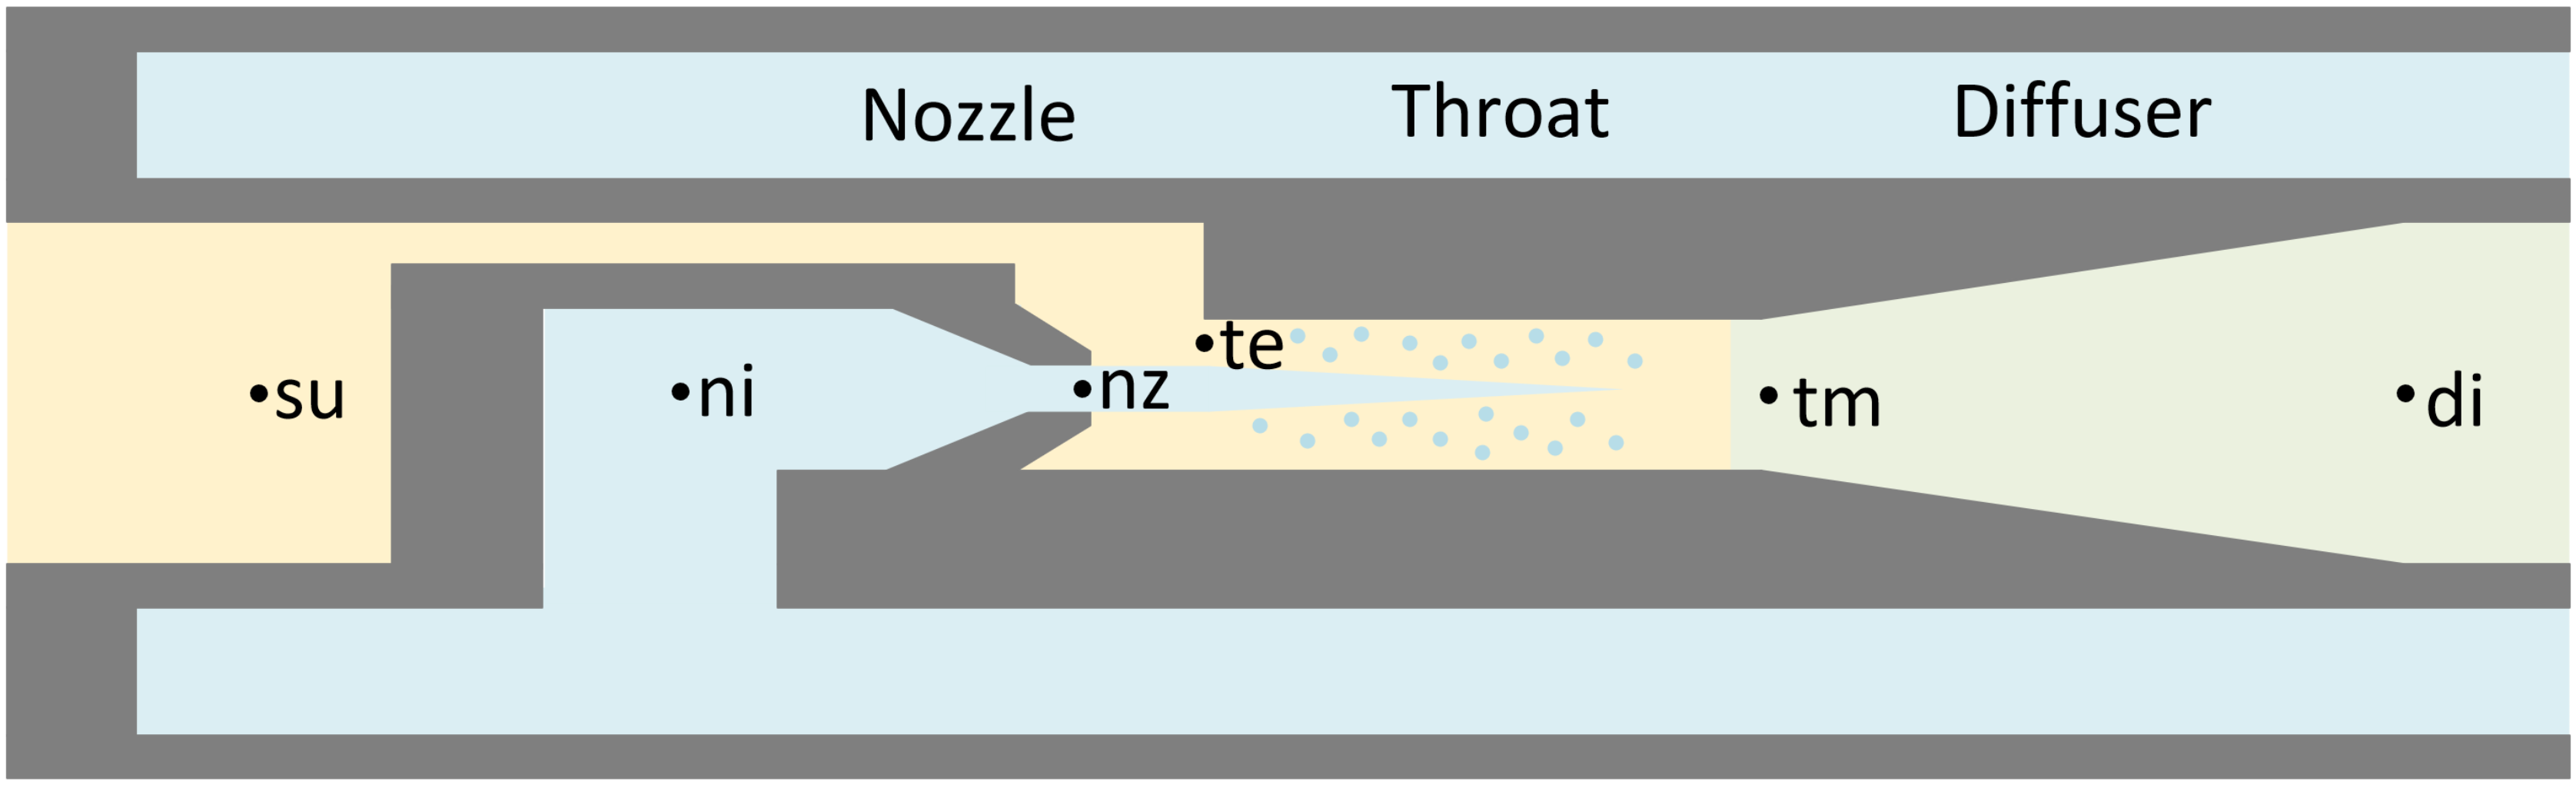
\includegraphics[width=1\linewidth]{figures/jetpump_ovr1.png}
    \caption{Jet Pump Overview}
    \label{fig:jetpump_side}
\end{figure}

\section{Energy Equation}

The one dimensional fluids energy equation \eqref{raw_energy} provides the foundation for compressible flow in conduits \cite{fluids_cheme}. The energy equation states that the differences in potential energy, pressure energy, kinetic energy, friction and work have to be equal.

\begin{equation}
gdz + \frac{dP}{\rho} + vdv + dF = dW
\label{raw_energy}
\end{equation}

For a jet pump, the potential energy and work terms can be omitted. The equation simplifies to the jet pump energy equation \eqref{jpump_energy}.

\begin{equation}
\frac{dP}{\rho} + vdv + dF = 0
\label{jpump_energy}
\end{equation}

Fluid flow across the nozzle tip, throat entrance and diffuser can all be modeled using variations of the jet pump energy equation. The most complex fluid dynamics occur in throat entrance and it has the biggest impact on jet pump performance.

\section{Throat Entrance}

The throat entrance is the area where the reservoir fluid flows into the throat. The power fluid is a solid jet at this location \cite{cunn_break}, taking away available flow area for the reservoir fluid. The jet pump energy equation is rewritten as differential energy equation for the throat entrance \eqref{diff_entr}. The suction velocity is assumed to be negligible.

\begin{equation}
dE_{te} = \int_{su}^{te} \frac{dP}{\rho} + \frac{v_{te}^{2}}{2} * (1+K_{en}) = 0
\label{diff_entr}
\end{equation}

The reservoir fluid behaves as a non-ideal gas, the oil is gas soluble and compressible. The mathematical model and analytical integration of such a complex fluid is difficult, if not impossible. To simplify the problem the analytical integral is transformed to a numerical integral with the trapezoid rule \eqref{trap_entr}.

\begin{equation}
dE_{te} = \frac{\Delta P}{2}\sum_{k=su}^{te} (\frac{1}{\rho_{k}} + \frac{1}{\rho_{k+1}}) + \frac{v_{te}^{2}}{2} * (1+K_{en}) = 0
\label{trap_entr}
\end{equation}

The throat entry differential energy equation is assessed in two sections, the pressure energy and the kinetic energy. The pressure energy is the area under the fluid specific volume curve. The kinetic energy is the throat entry velocity squared, distributed to account for the entrance friction. A solution is found when the sum of the pressure and kinetic energy equal zero. The method begins with a known suction pressure and oil mixture flow rate, defined by the wells inflow performance relationship (IPR). The pressure at the throat entrance is reduced in increments, driving new values of the kinetic and pressure energy. When the sum of these two terms equals zero, a solution is found and the reduction stops. Occasionally the reservoir fluid will hit its sonic velocity before the $dE_{te}$ equals zero. This implies too much flow is trying to be pushed through the jet pump throat entrance. A new higher suction pressure needs to be selected, which drives a lower reservoir flow rate. The next section provides further detail on the sonic velocity.

\section{Sonic Velocity}

Sonic velocity is defined as the max velocity that a sound wave can propagate through a fluid. Said in a another manner, its how quickly particles of a fluid can move through space before an accumulation of the particles occurs. Attempting to flow a fluid faster than its sonic velocity creates a build up of the fluid, which regulates the fluid speed down to the sonic velocity. The exception to this is when a specialized super sonic nozzle is used, allowing the particles to spread out which accelerates them above the sonic velocity. A super sonic nozzle cannot be designed into an oil well jet pump.

The sonic velocity limitation is exacerbated by a two-phase liquid and vapor mixture. The resultant sonic velocity of a two phase mixture is less than its individual components \cite{himr}. An example being a mixture of air and water. Individually the sonic velocity of the water and air are 5000 and 1100 ft/s respectively. Combining these fluids in a 50/50 mixture results in a sonic velocity of 300 ft/s.

Calculating the sonic velocity of an oil mixture is straight forward. A homogenous three phase mixture of oil, water and gas is assumed. The mixture bulk modulus of elasticity and density are calculated with equation \eqref{mix_elas} and \eqref{mix_dens} respectively.

\begin{equation}
\frac{1}{K_{mix}} = \frac{y_{o}}{K_{o}} + \frac{y_{w}}{K_{w}} + \frac{y_{g}}{K_{g}}
\label{mix_elas}
\end{equation}

\begin{equation}
\frac{1}{\rho_{mix}} = \frac{m_{o}}{\rho_{o}} + \frac{m_{w}}{\rho_{w}} + \frac{m_{g}}{\rho_{g}}
\label{mix_dens}
\end{equation}

\begin{equation}
c_{mix} = \sqrt{\frac{K_{mix}}{\rho_{mix}}}
\label{speed_sound}
\end{equation}

Another aspect that is made difficult by the sonic velocity is calculating when the $dE_{te}$ will cross the zero axis. When the fluid is operating sub sonic, or under a Mach value of 0.8, the relationship of $dE_{te}$ versus pressure is linear. As the fluid speeds up above mach 0.8, the slope of $dE_{te}$ against pressure starts to level off. When the fluid is operating at Mach One, the value of $\frac{dE_{te}}{dP}$ is zero. This is a known behavior in compressible fluid mechanics, where many relationships will flip in value once the fluid is super sonic \cite{fluids_white}. A derivation that analytically validates this behavior is show in the appendix and summarized in equation \eqref{dete_dp}. 

\begin{equation}
\frac{dE_{te}}{dp} = \frac{1}{\rho}(1 - \Mach^2)
\label{dete_dp}
\end{equation}

Areas of improvement:
Explain Mach numbers?

\printbibliography

\end{document}